\documentclass{../latex/utmreport}
\newcommand{\ReportTitle}{Lab 9: Watching System Calls with strace}
% Shared title-page and PDF metadata for every laboratory report.
\newcommand{\StudentName}{Gafenco Victor}
\newcommand{\StudentGroup}{FAF-241}
\newcommand{\CourseName}{Operating Systems}
\newcommand{\InstructorName}{Patricia Reițman}
\newcommand{\InstructorTitle}{Assistant lecturer}
\newcommand{\ReportCity}{Chișinău}
\newcommand{\ReportYear}{2026}
\newcommand{\CourseRepository}{https://github.com/yoda-dinmd/os-labs}

\selectlanguage{english}
\utmlogo{../latex/assets/UTM_Logo_English.jpeg}
\institution{Technical University of Moldova}
\faculty{Faculty of Computers, Informatics, and Microelectronics}
\department{Department of Software Engineering}
\studyprogramme{Software Engineering Study Programme}
\documenttype{Laboratory report}
\student{\StudentName}{\StudentGroup}
\supervisor{\InstructorName}{\InstructorTitle}
\renewcommand{\UTMCoordinatorLabel}{Instructor}
\cityyear{\ReportCity}{\ReportYear}
\reportsubtitle{\CourseName}
\hypersetup{pdfauthor={\StudentName},pdfsubject={\CourseName},
  pdftitle={\ReportTitle}}
\reporttitle{\ReportTitle}
\addto\captionsenglish{\renewcommand{\figurename}{Figure}\renewcommand{\tablename}{Table}\renewcommand{\bibname}{References}}
\renewcommand{\figurename}{Figure}
\renewcommand{\tablename}{Table}
\renewcommand{\bibname}{References}
\usepackage{float}
\usepackage{placeins}
\setlength{\emergencystretch}{2em}
\newcommand{\code}[1]{\texttt{\detokenize{#1}}}
% Keep screenshots beside their observations, with bounded height and width.
\newcommand{\screenshot}[4][\textwidth]{%
  \begin{figure}[H]
    \centering
    \includegraphics[width=#1,height=0.62\textheight,keepaspectratio]{screenshots/#2}
    \caption{#3}\label{#4}
  \end{figure}}
\newcommand{\reportreferences}[2]{%
  \clearpage\phantomsection\addcontentsline{toc}{chapter}{References}
  \begin{thebibliography}{9}
    \bibitem{handout} Technical University of Moldova, FCIM / FAF.
    \textit{#1}. Operating Systems laboratory handout, academic year 2026--2027.
    Supplied course document: \code{#2}.
  \end{thebibliography}}

\providecommand{\tightlist}{\setlength{\itemsep}{0pt}\setlength{\parskip}{0pt}}
\begin{document}
\makeutmreporttitlepage
\tableofcontents
\clearpage
\begin{utmabstract}[Abstract]
The goal of this laboratory is to observe and analyze the system-call boundary between user-space processes and the Linux kernel using \texttt{strace}. In Part~1, \texttt{strace} is used to trace \texttt{ls -l} while filtering \texttt{openat}, \texttt{read}, \texttt{write}, and \texttt{close}, identifying how standard utilities load shared libraries, read directory and user metadata, and write output to file descriptor~1. In Part~2, a C program (\texttt{syscalls.c}) directly invokes \texttt{open}, \texttt{write}, \texttt{read}, and \texttt{close} without \texttt{stdio} file buffering, demonstrating kernel file-descriptor allocation starting at descriptor~3. In Part~3, individual system call types are counted and compared using both single-call filtering (\texttt{strace -e trace=... | grep -c}) and kernel-call summary profiling (\texttt{strace -c}).
\utmkeywords{Linux, system calls, strace, openat, read, write, close, file descriptors, syscall profiling}
\end{utmabstract}
\utmintroduction

\section*{Goal of the laboratory (Scopul lucrării)}

The purpose of this laboratory work is to cross and inspect the boundary between user-space programs and the operating system kernel—the system call interface—on a real Linux system using \texttt{strace}. Specifically, the objectives are:
\begin{enumerate}
\tightlist
\item \textbf{Part 1 (See the calls of a real command):} Run \texttt{strace} on \texttt{ls -l} to observe the sequence of \texttt{openat}, \texttt{read}, \texttt{write}, and \texttt{close} system calls performed during program startup, directory reading, and terminal output, and identify which system call and file descriptor \texttt{ls} uses to print to the screen.
\item \textbf{Part 2 (A program that calls the kernel directly):} Write, compile, and trace a C program (\texttt{syscalls.c}) that creates a file, writes a string to it, and reads it back using only the \texttt{open}, \texttt{write}, \texttt{read}, and \texttt{close} system calls, and explain why the kernel assigns file descriptor~3.
\item \textbf{Part 3 (Count one kind of call):} Count how many times a program invokes a single kind of system call using both \texttt{strace -e trace=<syscall> ... | grep -c} and \texttt{strace -c}, and explain how output buffering and failed file probes affect individual call counts.
\end{enumerate}

All experiments were carried out on Linux (openSUSE Tumbleweed, x86\_64) using GCC with \texttt{-Wall -Wextra}. Complete trace logs and command outputs are recorded in \texttt{evidence/} and \texttt{report.md}.

\chapter{Part 1: See the calls of a real command}

\section{Running \texttt{strace} on \texttt{ls -l}}

To observe how a standard command interacts with the kernel, \texttt{ls -l} was executed under \texttt{strace} with the filter \texttt{-e trace=openat,read,write,close}:

\begin{lstlisting}
$ strace -f -e trace=openat,read,write,close ls -l
openat(AT_FDCWD, "/etc/ld.so.cache", O_RDONLY|O_CLOEXEC) = 3
close(3)                                = 0
openat(AT_FDCWD, "/lib64/libselinux.so.1", O_RDONLY|O_CLOEXEC) = 3
read(3, "\177ELF\2\1\1\0\0\0\0\0\0\0\0\0\3\0>\0\1\0\0\0\0\0\0\0\0\0\0\0"..., 1024) = 1024
close(3)                                = 0
openat(AT_FDCWD, "/lib64/libcap.so.2", O_RDONLY|O_CLOEXEC) = 3
read(3, "\177ELF\2\1\1\0\0\0\0\0\0\0\0\0\3\0>\0\1\0\0\0\300\214\0\0\0\0\0\0"..., 1024) = 1024
close(3)                                = 0
openat(AT_FDCWD, "/lib64/libc.so.6", O_RDONLY|O_CLOEXEC) = 3
read(3, "\177ELF\2\1\1\3\0\0\0\0\0\0\0\0\3\0>\0\1\0\0\0\256\267\2\0\0\0\0\0"..., 1024) = 1024
close(3)                                = 0
openat(AT_FDCWD, "/lib64/libpcre2-8.so.0", O_RDONLY|O_CLOEXEC) = 3
read(3, "\177ELF\2\1\1\0\0\0\0\0\0\0\0\0\3\0>\0\1\0\0\0\0\0\0\0\0\0\0\0"..., 1024) = 1024
close(3)                                = 0
openat(AT_FDCWD, "/usr/lib/locale/locale-archive", O_RDONLY|O_CLOEXEC) = -1 ENOENT (No such file or directory)
openat(AT_FDCWD, "/usr/share/locale/locale.alias", O_RDONLY|O_CLOEXEC) = 3
read(3, "# Locale name alias data base.\n#"..., 4096) = 2940
read(3, "", 4096)                       = 0
close(3)                                = 0
...
openat(AT_FDCWD, ".", O_RDONLY|O_NONBLOCK|O_CLOEXEC|O_DIRECTORY) = 3
close(3)                                = 0
openat(AT_FDCWD, "/etc/nsswitch.conf", O_RDONLY|O_CLOEXEC) = 4
read(4, "#\n# /etc/nsswitch.conf\n#\n# An ex"..., 4096) = 1221
read(4, "", 4096)                       = 0
close(4)                                = 0
openat(AT_FDCWD, "/etc/passwd", O_RDONLY|O_CLOEXEC) = 4
read(4, "root:x:0:0:root:/root:/bin/bash\n"..., 4096) = 1979
close(4)                                = 0
openat(AT_FDCWD, "/etc/group", O_RDONLY|O_CLOEXEC) = 4
read(4, "root:x:0:\nbin:x:1:daemon\ndaemon:"..., 4096) = 853
close(4)                                = 0
...
write(1, "total 416\n", 10total 416
)             = 10
openat(AT_FDCWD, "/etc/localtime", O_RDONLY|O_CLOEXEC) = 3
read(3, "TZif2\0\0\0\0\0\0\0\0\0\0\0\0\0\0\0\0\0\0\20\0\0\0\20\0\0\0\0"..., 4096) = 2424
read(3, "TZif2\0\0\0\0\0\0\0\0\0\0\0\0\0\0\0\0\0\0\20\0\0\0\20\0\0\0\0"..., 4096) = 1509
close(3)                                = 0
write(1, "-rw-r--r--. 1 victor victor   40"..., 57-rw-r--r--. 1 victor victor   4033 Nov  8 21:00 lab9.tex
) = 57
write(1, "-rw-r--r--. 1 victor victor    7"..., 57-rw-r--r--. 1 victor victor    783 Nov  8 21:01 notes.md
) = 57
write(1, "-rw-r--r--. 1 victor victor     "..., 57-rw-r--r--. 1 victor victor     14 Nov  8 13:33 note.txt
) = 57
write(1, "-rw-r--r--. 1 victor victor 3604"..., 57-rw-r--r--. 1 victor victor 360410 Nov  8 12:42 pic1.png
) = 57
write(1, "-rw-r--r--. 1 victor victor  211"..., 57-rw-r--r--. 1 victor victor  21159 Nov  8 13:33 pic2.png
) = 57
write(1, "-rw-r--r--. 1 victor victor    6"..., 58-rw-r--r--. 1 victor victor    693 Nov  8 21:00 README.md
) = 58
write(1, "-rwxr-xr-x. 1 victor victor  204"..., 57-rwxr-xr-x. 1 victor victor  20400 Nov  8 12:50 syscalls
) = 57
write(1, "-rw-r--r--. 1 victor victor    9"..., 59-rw-r--r--. 1 victor victor    984 Nov  8 12:47 syscalls.c
) = 59
close(1)                                = 0
close(2)                                = 0
+++ exited with 0 +++
\end{lstlisting}

\begin{figure}[H]
\centering
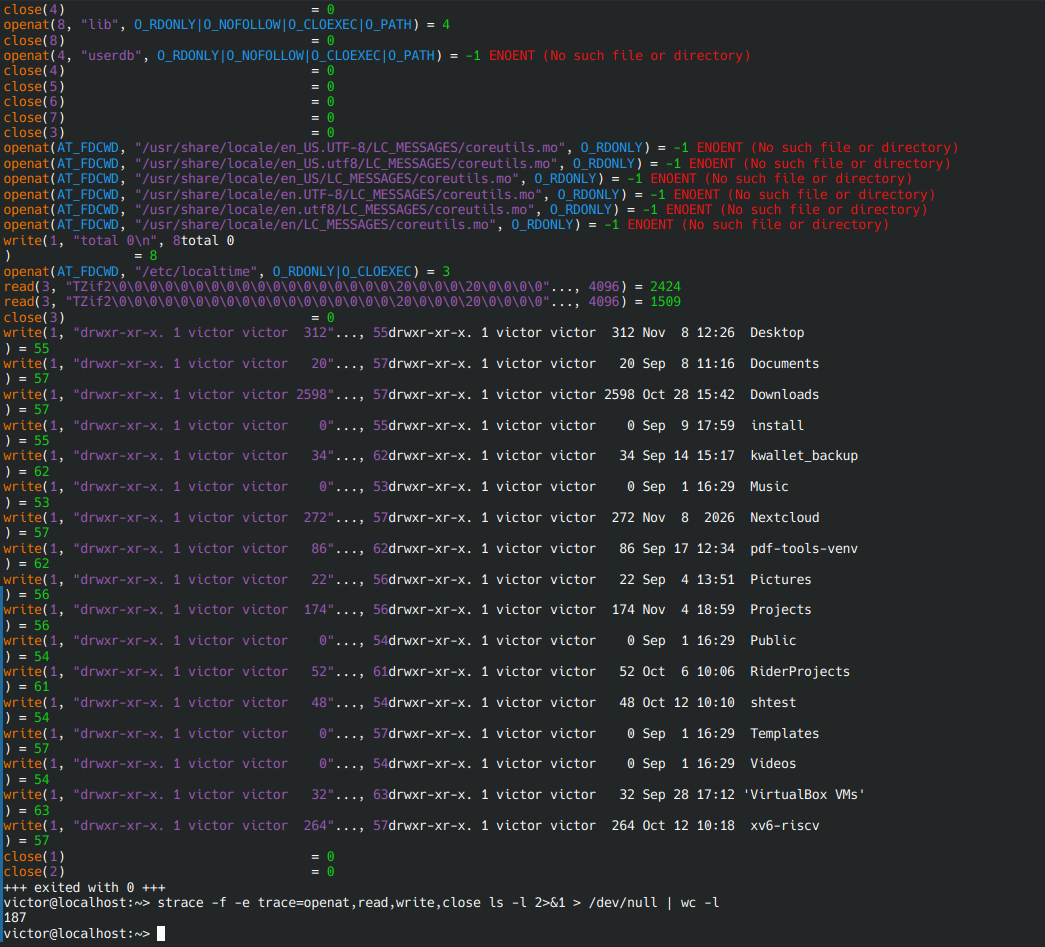
\includegraphics[width=0.96\linewidth]{pic1.png}
\caption{Terminal trace of \texttt{strace -f -e trace=openat,read,write,close ls -l}}
\end{figure}

\section{Observations for Part 1}

\begin{enumerate}
\tightlist
\item \textbf{Which system call does \texttt{ls} use to print to the screen? To which descriptor does it write?}
\texttt{ls} uses the \texttt{write} system call (\texttt{write(1, ..., ...)}) to print the formatted directory listing to the screen. It writes to \textbf{file descriptor~1}, which is \textbf{standard output (\texttt{stdout})}. When \texttt{stdout} is connected to a terminal, the C standard library uses line buffering, so each line of the \texttt{ls -l} listing is emitted via a separate \texttt{write(1, ...)} call.
\item \textbf{How many system calls does one simple \texttt{ls -l} make, roughly, and what happens during the trace?}
Even for a single directory, \texttt{ls -l} makes roughly \textbf{174--186 calls} among the four filtered types (\texttt{openat}, \texttt{read}, \texttt{write}, \texttt{close}) and \textbf{368--371 total system calls} when all system call types are included. The trace unfolds in four phases:
\begin{itemize}
\tightlist
\item \emph{Dynamic linker setup:} opening and reading ELF headers from \texttt{/etc/ld.so.cache}, \texttt{libselinux.so.1}, \texttt{libcap.so.2}, \texttt{libc.so.6}, and \texttt{libpcre2-8.so.0};
\item \emph{Locale configuration:} opening \texttt{LC\_*} locale files and probing optional message catalogs (\texttt{coreutils.mo}), where missing optional catalogs return \texttt{-1 ENOENT};
\item \emph{Directory and account lookup:} opening the target directory \texttt{"."} with \texttt{O\_DIRECTORY}, reading \texttt{/etc/nsswitch.conf}, \texttt{/etc/passwd}, \texttt{/etc/group}, and \texttt{/etc/localtime} to convert numeric UIDs, GIDs, and timestamps into human-readable strings;
\item \emph{Output and cleanup:} writing each line to descriptor~1 with \texttt{write(1, ...)} and closing descriptors~1 and~2 before exiting.
\end{itemize}
\end{enumerate}

\chapter{Part 2: A program that calls the kernel directly}

\section{Source code and execution of \texttt{syscalls.c}}

The program \texttt{syscalls.c} creates \texttt{note.txt}, writes a 14-byte string (\texttt{"hello, kernel\textbackslash n"}) directly through the kernel using \texttt{write}, closes the descriptor, reopens \texttt{note.txt} read-only, and reads the bytes back using \texttt{read}:

\begin{lstlisting}[language=C]
#include <fcntl.h>   /* open */
#include <unistd.h>  /* write, read, close */
#include <string.h>  /* strlen */
#include <stdio.h>   /* printf */

int main(void) {
    const char *msg = "hello, kernel\n";

    /* open() is a system call: ask the kernel for a file, get back a descriptor */
    int fd = open("note.txt", O_CREAT | O_WRONLY | O_TRUNC, 0644);
    if (fd < 0) { perror("open"); return 1; }
    printf("open returned descriptor %d\n", fd);

    /* write() is a system call: hand the bytes to the kernel */
    ssize_t n = write(fd, msg, strlen(msg));
    printf("write sent %zd bytes\n", n);
    close(fd);

    /* read it back, through the kernel again */
    fd = open("note.txt", O_RDONLY);
    char buf[64];
    n = read(fd, buf, sizeof(buf) - 1);
    buf[n] = '\0';
    printf("read got %zd bytes: %s", n, buf);
    close(fd);
    return 0;
}
\end{lstlisting}

Compiling and running \texttt{syscalls.c} produces the expected output:

\begin{lstlisting}
$ gcc -Wall -Wextra -o syscalls syscalls.c
$ ./syscalls
open returned descriptor 3
write sent 14 bytes
read got 14 bytes: hello, kernel
\end{lstlisting}

\begin{figure}[H]
\centering
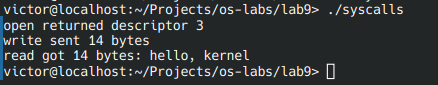
\includegraphics[width=0.85\linewidth]{pic2.png}
\caption{Execution of the direct system-call program \texttt{./syscalls}}
\end{figure}

\section{Tracing \texttt{./syscalls} with \texttt{strace}}

Running \texttt{strace -e trace=openat,write,read,close ./syscalls} shows both the dynamic loader setup and our six direct file system calls:

\begin{lstlisting}
$ strace -e trace=openat,write,read,close ./syscalls
openat(AT_FDCWD, "/etc/ld.so.cache", O_RDONLY|O_CLOEXEC) = 3
close(3)                                = 0
openat(AT_FDCWD, "/lib64/libc.so.6", O_RDONLY|O_CLOEXEC) = 3
read(3, "\177ELF\2\1\1\3\0\0\0\0\0\0\0\0\3\0>\0\1\0\0\0\256\267\2\0\0\0\0\0"..., 1024) = 1024
close(3)                                = 0
openat(AT_FDCWD, "note.txt", O_WRONLY|O_CREAT|O_TRUNC, 0644) = 3
write(1, "open returned descriptor 3\n", 27open returned descriptor 3
) = 27
write(3, "hello, kernel\n", 14)         = 14
write(1, "write sent 14 bytes\n", 20write sent 14 bytes
)   = 20
close(3)                                = 0
openat(AT_FDCWD, "note.txt", O_RDONLY)  = 3
read(3, "hello, kernel\n", 63)          = 14
write(1, "read got 14 bytes: hello, kernel"..., 33read got 14 bytes: hello, kernel
) = 33
close(3)                                = 0
+++ exited with 0 +++
\end{lstlisting}

\section{Observations for Part 2}

\begin{itemize}
\tightlist
\item \textbf{The descriptor returned by the first \texttt{openat} is 3, not 0, 1 or 2. Why are those three already taken?}
Every POSIX process inherits three pre-opened standard stream descriptors from its parent shell when started:
\begin{itemize}
\tightlist
\item Descriptor \textbf{0}: standard input (\texttt{stdin}, \texttt{STDIN\_FILENO}),
\item Descriptor \textbf{1}: standard output (\texttt{stdout}, \texttt{STDOUT\_FILENO}),
\item Descriptor \textbf{2}: standard error (\texttt{stderr}, \texttt{STDERR\_FILENO}).
\end{itemize}
Because the Linux kernel always allocates the \textbf{lowest-numbered unused file descriptor} in the process's file descriptor table, the first call to \texttt{open("note.txt", ...)} (implemented by glibc via the \texttt{openat} system call relative to \texttt{AT\_FDCWD}) returns descriptor~\textbf{3}. When \texttt{close(3)} is called after writing, descriptor~3 becomes free again, so the second \texttt{open("note.txt", O\_RDONLY)} immediately reuses descriptor~\textbf{3}.
\end{itemize}

\chapter{Part 3: Count one kind of call}

\section{Counting individual system call types with \texttt{strace -e trace=... | grep -c}}

Whereas piping a multi-call trace to \texttt{wc -l} counts all displayed lines combined (including the \texttt{+++ exited with 0 +++} status line), counting a \textbf{single kind of system call} requires either filtering a single system call with \texttt{-e trace=<syscall>} and counting matching lines with \texttt{grep -c}, or using \texttt{strace -c}.

Running \texttt{strace -e trace=<syscall>} with \texttt{grep -c} on \texttt{ls -l} for each of the four system calls individually:

\begin{lstlisting}
$ strace -e trace=openat ls -l 2>&1 >/dev/null | grep -c '^openat'
102
$ strace -e trace=close ls -l 2>&1 >/dev/null | grep -c '^close'
56
$ strace -e trace=read ls -l 2>&1 >/dev/null | grep -c '^read'
15
$ strace -e trace=write ls -l 2>&1 >/dev/null | grep -c '^write'
1
\end{lstlisting}

Doing the same single-call count on \texttt{./syscalls}:

\begin{lstlisting}
$ strace -e trace=openat ./syscalls 2>&1 >/dev/null | grep -c '^openat'
4
$ strace -e trace=close ./syscalls 2>&1 >/dev/null | grep -c '^close'
4
$ strace -e trace=read ./syscalls 2>&1 >/dev/null | grep -c '^read'
2
$ strace -e trace=write ./syscalls 2>&1 >/dev/null | grep -c '^write'
2
\end{lstlisting}

In \texttt{./syscalls}, the 4 \texttt{openat} and 4 \texttt{close} calls consist of 2 library loads (\texttt{/etc/ld.so.cache} and \texttt{libc.so.6}) plus our 2 opens/closes of \texttt{note.txt}. The 2 \texttt{read} calls are 1 ELF header read of \texttt{libc.so.6} plus our \texttt{read(3, ...)} from \texttt{note.txt}. The 2 \texttt{write} calls are our unbuffered \texttt{write(3, "hello, kernel\textbackslash n", 14)} plus 1 buffered \texttt{write(1, ...)} flushing all three \texttt{printf} lines at exit when \texttt{stdout} is redirected to \texttt{/dev/null}.

\section{Summary profiling per system call with \texttt{strace -c}}

The built-in \texttt{strace -c} option counts invocations, errors, and kernel execution time for each system call type individually. Restricting \texttt{strace -c} to the four calls from Part~1:

\begin{lstlisting}
$ strace -c -e trace=openat,read,write,close ls -l >/dev/null
% time     seconds  usecs/call     calls    errors syscall
------ ----------- ----------- --------- --------- ----------------
 72.06    0.000539           5       102        48 openat
 21.66    0.000162           2        56           close
  6.02    0.000045           3        15           read
  0.27    0.000002           2         1           write
------ ----------- ----------- --------- --------- ----------------
100.00    0.000748           4       174        48 total
\end{lstlisting}

Running \texttt{strace -c ls -l >/dev/null} without a filter counts every distinct system call type made by \texttt{ls -l}:

\begin{lstlisting}
$ strace -c ls -l >/dev/null
% time     seconds  usecs/call     calls    errors syscall
------ ----------- ----------- --------- --------- ----------------
 34.95    0.001475          14       102        48 openat
 14.31    0.000604          14        43           mmap
  8.70    0.000367         367         1           execve
  7.68    0.000324           5        56           close
  5.71    0.000241           6        35           statx
  4.83    0.000204          10        20           newfstatat
  4.15    0.000175          21         8           mprotect
  4.03    0.000170           5        31           fstat
  3.15    0.000133           8        15           read
  2.30    0.000097          10         9           llistxattr
  1.82    0.000077          25         3         2 access
  1.54    0.000065           7         9           lgetxattr
  0.90    0.000038           4         8           lseek
  0.81    0.000034           5         6         4 prctl
  0.78    0.000033          16         2           getdents64
  0.76    0.000032          16         2         2 ioctl
  0.76    0.000032          16         2           statfs
  0.55    0.000023           5         4           futex
  0.50    0.000021           7         3           brk
  0.45    0.000019           4         4           rt_sigprocmask
  0.40    0.000017           8         2           getrandom
  0.36    0.000015          15         1           prlimit64
  0.14    0.000006           6         1           arch_prctl
  0.14    0.000006           6         1           set_tid_address
  0.14    0.000006           6         1           set_robust_list
  0.14    0.000006           6         1           rseq
  0.00    0.000000           0         1           write
------ ----------- ----------- --------- --------- ----------------
100.00    0.004220          11       371        56 total
\end{lstlisting}

\begin{figure}[H]
\centering
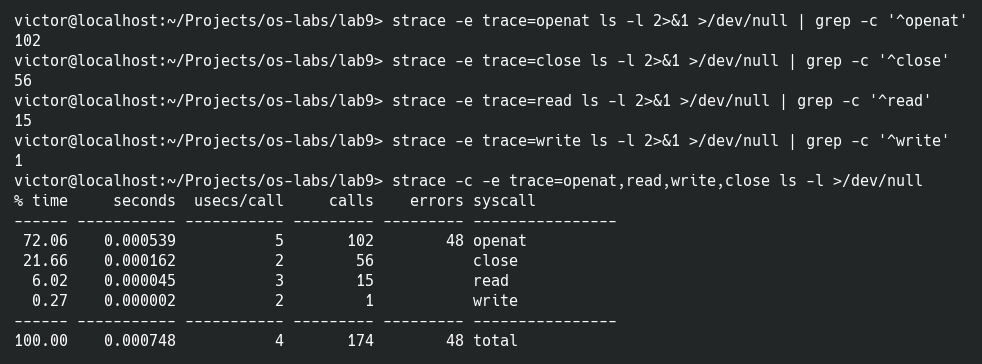
\includegraphics[width=0.95\linewidth]{pic3.png}
\caption{Counting individual system call types with \texttt{strace -e trace=... | grep -c} and \texttt{strace -c}}
\end{figure}

\section{Observations for Part 3}

\begin{enumerate}
\tightlist
\item \textbf{Matching \texttt{openat} and \texttt{close} counts:}
Out of \textbf{102} \texttt{openat} calls, \textbf{48} return \texttt{-1 ENOENT} (failed lookups for optional locale catalogs and userdb sockets), leaving $102 - 48 = 54$ successful opens that allocate file descriptors. Adding the closing of standard output (\texttt{close(1)}) and standard error (\texttt{close(2)}) before exit yields $54 + 2 = \mathbf{56}$ \texttt{close} calls.
\item \textbf{Effect of standard output buffering on \texttt{write} count:}
When \texttt{ls -l} outputs directly to the terminal (Part~1), \texttt{glibc} detects a terminal via \texttt{ioctl(1, TCGETS, ...)} and configures \texttt{stdout} as line-buffered, resulting in one \texttt{write(1, ...)} call per output line (9 \texttt{write} calls for 8 files plus the \texttt{total} line). When \texttt{stdout} is redirected to \texttt{/dev/null}, \texttt{ioctl} returns \texttt{ENOTTY} and \texttt{glibc} switches to a 4096-byte block buffer, coalescing all output lines into a single \texttt{write(1, ..., 469)} call.
\end{enumerate}

\utmconclusions

Using \texttt{strace}, this laboratory observed the Linux system-call interface from three perspectives:
\begin{itemize}
\tightlist
\item In \textbf{Part~1}, tracing \texttt{ls -l} showed how a real utility loads shared libraries, queries locale and account databases, and prints to the screen via \texttt{write} on file descriptor~1 (\texttt{stdout}).
\item In \textbf{Part~2}, writing and tracing \texttt{syscalls.c} confirmed that \texttt{open}, \texttt{write}, \texttt{read}, and \texttt{close} cross directly into the kernel and that the first opened file receives descriptor~3 because descriptors~0, 1, and~2 are already occupied by \texttt{stdin}, \texttt{stdout}, and \texttt{stderr}.
\item In \textbf{Part~3}, counting single system call types with \texttt{strace -e trace=<call> ... | grep -c} and \texttt{strace -c} quantified the exact per-call breakdown for \texttt{ls -l} (102 \texttt{openat}, 56 \texttt{close}, 15 \texttt{read}, and 1 block-buffered \texttt{write} out of 371 total system calls) and explained the relationship between successful \texttt{openat} calls, \texttt{close} calls, and \texttt{stdio} buffering.
\end{itemize}
\end{document}
